% Test, že co jsem udělal já funguje
\chapter{Ověření funkčnosti návrhu ($\Sigma$ = 4 strany)}
Pro testování funkčnosti systému jsem zkusil celý systém nastavit přesně podle instrukcí obsažených v Setup stránce dostupné v mobilní aplikace. Poté jsem připojil celý systém na digitální vstupy do ovládacího panelu frekvenčního měniče a připojil jsem systém na napájecí napětí 24V OUT vycházející z ovládacího panelu. Jak jsem zkontroloval, že je všechno nastavené jak má být, otestoval jsem, jestli lokální ovládání spíná digitální vstupy ovládacího panelu. Po kontrole, že tomu tak je, je možné zapnout výkonovou část frekvenčního měniče (tedy část mimo ovládací panel). Tohle spustí dopravník.

Při zapínání výkonové části frekvenčního měniče je důležité si dát pozor, aby aproximace rychlosti začínala na nule, protože jinak bude začínat aproximaci na posunuté hodnotě.

Všechno testování bylo provedeno v Brněnské hale společnosti Honeywell. V té je rozmístěno několik různých typů dopravníkových linek které Honeywell Brno nabízí svým zákazníkům na fyzických i virtuálních prohlídkách. V době, kdy byla v hale testovaná funkčnost celého systému byla asi 80 metrů daleko v jiné části haly spuštěná jiná dopravníková linka, ale vzhledem k tomu, že vzdálenost dosahu WiFi signálu vyšla v rámci přijatelných mezí, lze předpokládat, že nebyla nijak druhou linkou zarušena. Je možné, že dosah bude v hale zákazníka jiný - to záleží podle dalších zdrojů rušení, hustoty dopravníků v dané oblasti a přítomnost dalších faktorů, které by mohly rušit WiFi vlny.

\begin{figure}
    \centering
    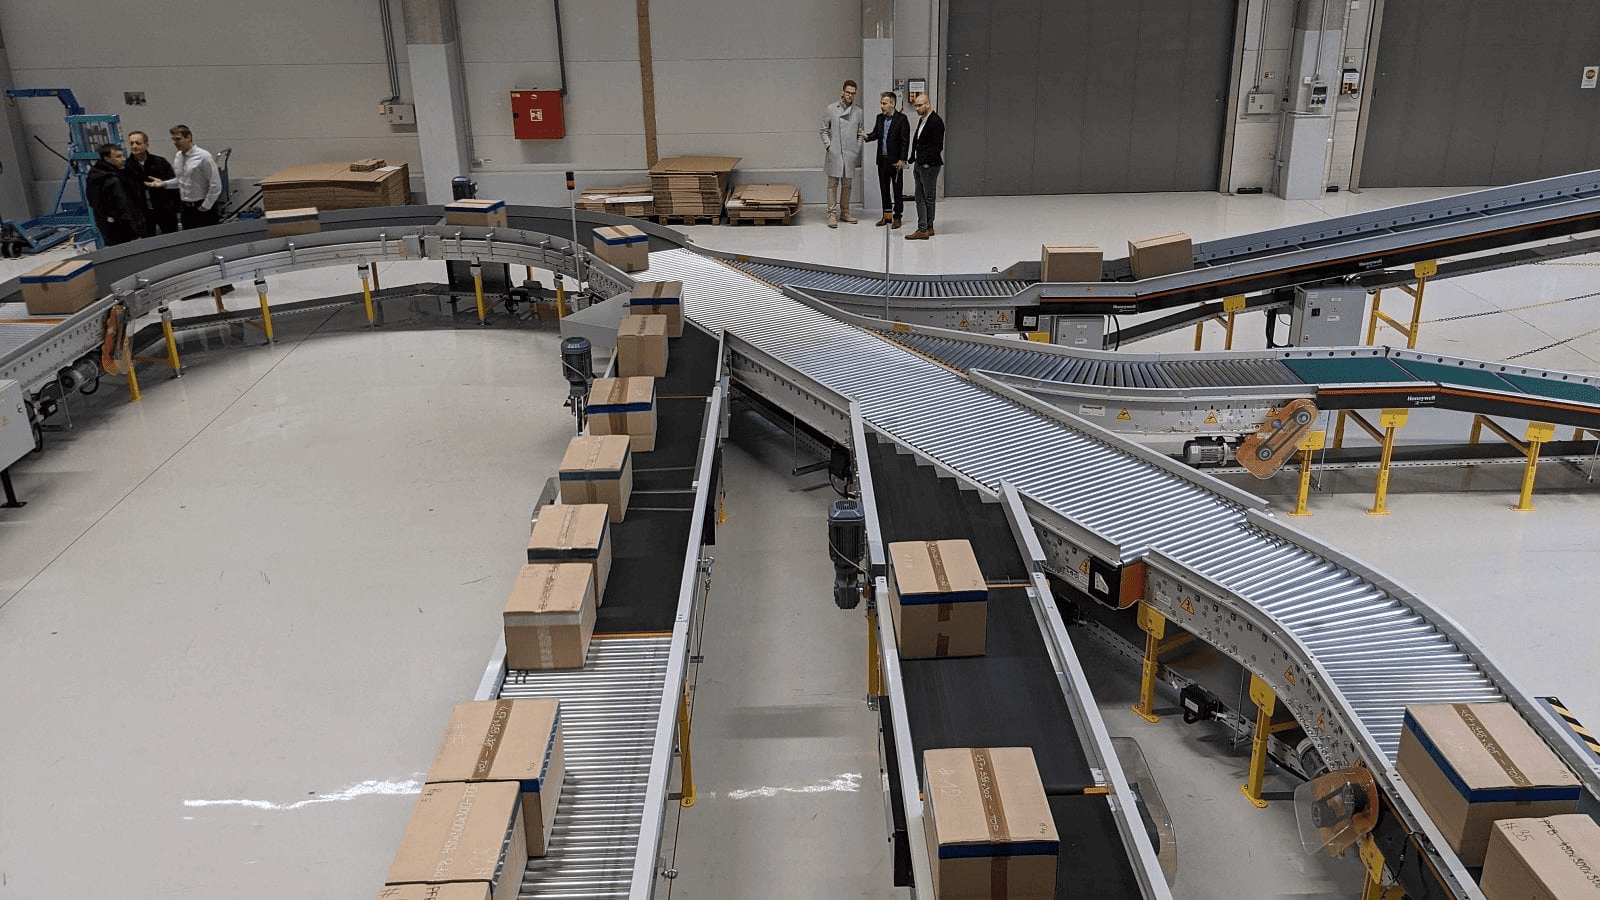
\includegraphics[width=1\linewidth]{images/BrnenskaHoneywellHala.png}
    \caption{Ukázka Brněnské haly pro testování dopravníků společnosti Honeywell \cite{HoneywellHala}}
    \label{fig:BrnenskaHoneywellHala}
\end{figure}

\section{Ověření funkčnosti lokálního ovládání (0.5 strany)}
\purpose{Tady bych se chtěl zaměřit na to, jestli je možné dopravník ovládat přes tlačítka rovnou umístěná na desce.}

Tohle jsem už testoval a funguje to jak má. Ty tlačítka spínají přímo těch 24V z ovládacího panelu dopravníku, takže fungují i když se vůbec nepřipojí ten mikrokontroller - tudíž deska funguje i bez připojení kabelu který vede na 24V OUT port, ale potom nefunguje LCD displej pro aproximaci rychlosti dopravníku.

\section{Ověření funkčnosti mobilní aplikace (1 strana)}
\purpose{Tady jenom potvrdím že mobilní aplikace opravdu funguje}

Po zapojení dopravníku a otestování lokálního ovládání byla testována mobilní aplikace.

Pro používání mobilní aplikace jsem zapnul systém do stavu pro dálkové ovládání. Do mobilní aplikace následně stačí pouze přidat IP adresu která je vidět na LCD displeji desky a kliknout tlačítko "Add Conveyor". Po přidání dopravníku do aplikace je možné spustit dopravník a po spuštění dopravník zrychlovat i zpomalovat. Aproximace rychlosti lze úspěšně vidět nad tlačítky pro ovládání dopravníku. Při ovládání dopravníku na dálku je také typ ovládání v aplikaci viditelný jako "Remote".

V rámci tohoto testu jsem šel na X metrů daleko a zkontroloval že ta deska funguje i na nějakou vzdálenost.

\section{Ověření funkčnosti zapojení více desek (0.5 strany)}
\purpose{Tady bych se rád zaměřil na nějaké testy, při kterých zkouším, jestli je opravdu možné ovládat víc desek zároveň.}

Pro otestování jsem nastavil a zapojil dvě desky podle návodu u dvou dopravníků několik metrů od sebe. Následně jsem testoval vzdálenost kde se mi podařilo si zachovat spojení s obouma deskami na X metrů. Tohle bylo znovu testované v Brněnské Honeywell hale. Při testování jsem sledoval jestli se dopravníky hýbou tím, že jsem si na dopravník položil testovací balík a u toho bylo vidět, jestli se při dané vzdálenosti hýbe anebo už ne.

\section{Posouzení z hlediska bezpečnosti (1 strana)}\label{sec:PosouzeniZHlediskaBezpecnosti}
\purpose{Tady bude nějaký moje zamyšlení nad bezpečností téhle desky. }

Ta deska už ze své podstaty má umožňovat ovládat dopravník na dálku a někdy i třeba hodinu - aby si sedly všechny součásti a tak bylo vidět, jestli je dopravník opravdu v pořádku za chodu. Tohle může být inherentně nebezpečná věc pokud by operátor přišel o spojení s deskou ve špatný okamžik a nemohl tak dopravník zastavit. Je možný, že by měla obsahovat nějakej test (třeba každou sekundu), jestli je otevřená aplikace na mobilu, ale to by kazilo user experience uživatelů, který dělají ty testy, protože oni musí při používání aplikace ještě psát informace o zkouškách do excelu. Pokud by se aplikace zavřela, tak přestane komunikovat s deskou a ta by pak chtěla ten dopravník vypnout. Tenhle bezpečnostní mechanismus tedy nemá smysl implementovat, protože by příliš kazil používání systému jako takového.

Myšlenku žádný takový mechanismus nevytvářet také podporuje fakt, že navržený systém přebírá bezpečnost z těch už nainstalovaných dopravníků. Dopravníky už při této fázi kontroly kvality mají kolem sebe E-STOP lanko a E-STOP tlačítka, které jsou nastavené aby dopravníku přikázali pohotovostní zastavení, jak vyžaduje bezpečnost na pracovišti.

V rámci bezpečnosti je také důležité správně vyškolit obsluhu systému pro bezpečné používání systému. Obsluha by měla například vědět, že je potřebné vypnout výkonovou část frekvenčního měniče pomocí nainstalovaného vypínače při veškeré manipulaci s ovládacím panelem. Obsluha by také měla vědět jak správně systém nastavit a jak řešit časté problémy - obě témata obsahuje mobilní aplikace na adresách Setup a Help.

% \section{Spolehlivost bezdrátové komunikace (0.5 strany)}
% \purpose{Tady bych rád otestoval, kolik metrů bude dosah WiFi ve skladu Honeywellu.}